% !TeX spellcheck = en_US
\documentclass[%
% DOCUMENT LAYOUT
a4paper,           % paper size
12pt,              % The default document font size, options: 10pt, 11pt, 12pt
onehalfspacing,    % onehalfspacing line spacing, alternatives: doublespacing, or singlespacing
nolistspacing,     % If the document is onehalfspacing or doublespacing, uncomment this to set spacing
		    	   % in lists to single
indentfirst,       % Uncomment to indent the first paragraph of each chapter/section/etc. 
parskip,           % Uncomment to add space between paragraphs
headsepline,       % Uncomment to get a line under the header
%chapterinoneline, % Uncomment to place the chapter title next to the number on one line
%consistentlayout, % Uncomment to change the layout of the declaration, abstract and 
                   % acknowledgements pages to match the default layout
liststotoc,		   % Uncomment to add the list of figures/tables/etc to the table of contents
toctotoc,          % Uncomment to add the main table of contents to the table of contents
%
% -----------------
% LANGUAGE SETUP <--- LOOK AT ME I'M VERY IMPORTANT!	
% -----------------	
{french,english},  % second, first -- USE IF YOU ARE WRITING YOUR THESIS IN ENGLISH
%{english,french}, % second, first -- USE IF YOU ARE WRITING YOUR THESIS IN FRENCH 
 -----------------
% EXTRA RESOURCES
% -----------------	
%nocleverefsupport, % Uncomment to not load the  clevref package (\Cref and \cref)
%nohyperrefsupport, % Uncomment to not load the hyperref package
%noacro,               % Uncomment to not load the acro package
% -----------------
% FOR DEBUGING     
% -----------------    
%draft, % Uncomment to enable draft mode (no pictures, no links, overfull hboxes indicated)
]{MathSTICUBL}
\usepackage[T1]{fontenc}
\usepackage[utf8]{inputenc}
\usepackage{mathpazo} % Use the Palatino font by default
%\usepackage[libertine,cmintegrals,cmbraces,vvarbb]{newtxmath}
%\usepackage[scaled=0.95]{inconsolata}
\usepackage{siunitx} % for unites 

% Used only for examples
\usepackage{blindtext}    % for this example file only
\usepackage{lipsum}       % for his example file only
\usepackage[Q=yes]{examplep} % for his example file only
%----------------

\usepackage{algorithmic} % you can use another.
%----------------------------------------------------------------------------------------
%	THESIS INFORMATION
%----------------------------------------------------------------------------------------
% Thesis number, provider by someone
\tnumber{00000}
%----------------------------------------------------------------------------------------
% Your {Name} {Surname} 
%----------------------------------------------------------------------------------------
\author{Prénom-Composé}{Nom-Composé}
%----------------------------------------------------------------------------------------

%----------------------------------------------------------------------------------------
% Your advisors (fisrt is the director) others: co-director
%----------------------------------------------------------------------------------------
\advisor[Mme]{Dr.\ Jeanne}{d'Arc}{Fonction ---  établissement d’exercice}
\advisor[Mme]{Dr.\ Ayrton}{Senna da Silva}{Fonction ---  établissement d’exercice}
%\advisor[M]{Dr.\ Blaise}{Pascal}{Fonction ---  établissement d’exercice}

%----------------------------------------------------------------------------------------
% Jury President
%----------------------------------------------------------------------------------------
\president[Mme]{Dr.\ Ada}{Lovelace}{Fonction ---  établissement d’exercice}

%----------------------------------------------------------------------------------------
% Jury Rapporteurs
%----------------------------------------------------------------------------------------
\rapporteur[M]{Dr.\ George}{Pompidou}{Fonction ---  établissement d’exercice}
\rapporteur[Mme]{Dr.\ Alain}{Prost}{Fonction ---  établissement d’exercice}
%\rapporteur[M]{Dr.\ George}{Pompidou}{Fonction ---  établissement d’exercice}
%\rapporteur[Mme]{Dr.\ Ada}{Lovelace}{Fonction ---  établissement d’exercice}
%----------------------------------------------------------------------------------------
% Jury Examinateur
%----------------------------------------------------------------------------------------
\examinateur[M]{Dr.\ Donald Ervin}{Knuth}{Fonction ---  établissement d’exercice}
\examinateur[M]{Dr.\ Leslie}{Lamport}{Fonction ---  établissement d’exercice}
%\examinateur[M]{Dr.\ George}{Pompidou}{Fonction ---  établissement d’exercice}
%\examinateur[Mme]{Dr.\ Ada}{Lovelace}{Fonction ---  établissement d’exercice}
%----------------------------------------------------------------------------------------
% Jury Invités
%----------------------------------------------------------------------------------------
\invite[M]{Dr.\ Ricardo}{Carlini}{Fonction ---  établissement d’exercice}

% Your school:
%\school{AGRO}% AGRO - Agrocampus Ouest
%\school{CS}    %    CS - Centrale Superlec
%\school{ECN}   %   ECN - Ecole Centrale Nantes
%\school{ENIB}  %  ENIB - Ecole Natiolane d'ingenieurs de Brest
%\school{ENS}   %   ENS - Ecole Normale Superieure
%\school{ENSAI} % ENSAI - École nationale de la statistique et de l'analyse de l'information   
%\school{ENSTA} % ENSTA - L’École nationale supérieure de techniques avancées Bretagne 
%\school{IMTA}  %  IMTA - L'École nationale supérieure Mines-Télécom Atlantique Bretagne Pays de la Loire.  
%\school{INSA}  %  INSA - L’institut national des sciences appliquées de Rennes 
%\school{LMU}   %   LMU - Le Mans Université
%\school{UA}    %    UA - Université d'Angers 
%\school{UBO}   %   UBO - Université de Bretagne Occidentale 
%\school{UBS}   %   UBS - Université de Bretagne Sud 
%\school{UN}    %    UN - Université de Nantes 
%\school{UR1}   %   UR1 - Université Rennes 1
%\school{UR2}   %   UR2 - Université Rennes 2 
% ENIB
\school{AGRO}
%----------------------------------------------------------------------------------------
% Look at https://theses.u-bretagneloire.fr/bs
\lab{IRISA --- UMR6074}
%----------------------------------------------------------------------------------------
% Look at https://theses.u-bretagneloire.fr/bs
\subject{voir liste des spécialités} % Informatique
%----------------------------------------------------------------------------------------
% In case of cotutle, we need to inform, the logo_path and the university name
\cotutele{logo-PUCMINAS}{Pontifícia Universidade Católica de Minas Gerais --- Brasil}
%----------------------------------------------------------------------------------------
% city
\city{Lieu}
%----------------------------------------------------------------------------------------
\date{\today}
%----------------------------------------------------------------------------------------
% If you wanna change the margins. Class default values: 
% A4 paper / 2.5 / 2.5 / 0.5 / 1.5 / 2.0 
%\geometry{%
%	paper=a4paper,      % Change to letterpaper for US letter
%	inner=3.0cm,        % Inner margin`
%	outer=2.0cm,        % Outer margin
%	bindingoffset=.5cm, % Binding offset
%	top=1.5cm,          % Top margin
%	bottom=2.0cm,       % Bottom margin
%	showframe,          % Uncomment to show how the type block is set on the page
%}

%----------------------------------------------------------------------------------------
% If your thesis is in French
%----------------------------------------------------------------------------------------
\title{Thesis Title}
\subtitle{Thesis subtitle}
\titre{Titre de la thèse}
\soustitre{Sous-titre de la thèse}


%----------------------------------------------------------------------------------------
% Abstract: 
%----------------------------------------------------------------------------------------
\abstract{%
	\foreignlanguage{english}{\blindtext[3]}
}
\keywords{from 3 to 6 keywords}

%----------------------------------------------------------------------------------------
\resume{% 
	\foreignlanguage{french}{\blindtext[3]}
}
\motscles{de 3 à 6 mots clefs}
%----------------------------------------------------------------------------------------


%\usepackage[backend=biber,style=authoryear,natbib=true]{biblatex} % Use the bibtex backend with the authoryear citation style (which resembles APA)


\addbibresource{example.bib} % The filename of the bibliography
%----------------------------------------------------------------------------------------1
% PUT HERE YOUR EXTRA PACKAGES
%----------------------------------------------------------------------------------------



%----------------------------------------------------------------------------------------
%  The document structure begins here!
%----------------------------------------------------------------------------------------
\begin{document}
\frontmatter%		 % Use roman page numbering style (i, ii, iii, iv...) for the pre-content pages
\maketitle%			 % make the cover 
\pagestyle{plain}	 % Default to the plain heading style until the thesis style is called for the body content
%----------------------------------------------------------------------------------------
%	QUOTATION PAGE
%----------------------------------------------------------------------------------------
\makequotation{Moving on, is a simple thing, what it leaves behind is hard}{Dave Mustaine}{\`{A} Tout le Monde}
%
%----------------------------------------------------------------------------------------
%	DEDICATION
%----------------------------------------------------------------------------------------
\dedicatory{à Julia et Fernanda} 

%----------------------------------------------------------------------------------------
%	Acknowledgements
%----------------------------------------------------------------------------------------
\begin{acknowledgements}
\addchaptertocentry{\acknowledgementname} % Add the acknowledgements to the table of contents
 \begin{spacing}{1.0} % cover is always 1 line spacing
{%\small
	Je remercie \PRESp\ \PRESn, \PRESq, qui me fait l'honneur 
	de présider ce jury.\\[\baselineskip]
	
	Je remercie %
	\setcounter{III}{1}%
	\whiledo{\value{III}<\value{nrap}}{%
		\pnqRAP{\roman{III}}%
		\stepcounter{III}%
		\ifthenelse{\value{III}=\value{nrap}}{, et }{, }%
	}\pnqRAP{\roman{nrap}}, d'avoir bien voulu accepter la charge 
	de rapporteur.\\[\baselineskip]
	
	Je remercie %
	\setcounter{III}{1}%
	\whiledo{\value{III}<\value{nexa}}{%
		\pnqEXA{\roman{III}}%
		\stepcounter{III}%
		\ifthenelse{\value{III}=\value{nexa}}{, et }{, }%
	}\pnqEXA{\roman{nexa}}, d'avoir bien voulu juger ce travail.\\[\baselineskip]
	
	Je remercie enfin %
		\setcounter{III}{1}%
	\whiledo{\value{III}<\value{nadv}}{%
		\pnqADV{\roman{III}}%
		\stepcounter{III}%
		\ifthenelse{\value{III}=\value{nadv}}{, et }{, }%
	}\pnqEXA{\roman{nadv}}, 
	qui  a dirigé ma thèse.\\[\baselineskip]
	
	\vfill
}
\end{spacing}
\end{acknowledgements}


%fim

\dominitoc
\setcounter{mtc}{2}   % To fix the minitoc content (before Résumé Étendú we have the acknow.)
%----------------------------------------------------------------------------------------
%	Resume Etendu en Francais (only if your thesis is in English)
%----------------------------------------------------------------------------------------
\ifcurrentbaselanguage{English}{%
	% !TeX spellcheck = fr_FR
\begin{otherlanguage}{french}
\addchap{Résumé Étendú}
\epigraph{Il vaut mieux faire que dire.}{Alfred de \textsc{Musset}}
\minitoc%
 %----------------------------------------------------------------------------------------------
Afin de garantir le respect des chartes graphiques des établissements et la cohérence du support, les  logos, les noms des établissements, le numéro de l’école doctorale, le nom de l’école doctorale, l’image de fond et le titre: Thèse de Doctorat ne sont pas modifiables.
%----------------------------------------------------------------------------------------------
\addsec{Instructions sur les paramètres modifiables}

\begin{enumerate}[label= (\arabic*)]
	\item Indiquer dans le cas d’une co-tutelle des 2 établissements de délivrance du diplôme (Docteur de établissement 1 Docteur de établissement 2)
	\item Si la thèse est en co-tutelle, mettre le logo des 2 établissements
	\item Indiquer la spécialité
	\item Attention: le prénom doit être en minuscules (Jean) et le \textsc{Nom} en majuscules (\textsc{Brittef})
	\item Donner le titre complet de la thèse, éventuellement le sous titre, si nécessaire sur plusieurs lignes
	\item Indiquer la date et le lieu de soutenance de la thèse
	\item Indiquer le nom du (ou des) laboratoire (s) dans le(s)quel(s) le travail de thèse a été effectué, indiquer aussi si souhaité le nom de la (les) faculté(s) (UFR, école(s), Institut(s), Centre(s)\ldots), son 	(leurs) adresse(s)\ldots
    \item Indiquer le N\textordmasculine{} de thèse, si cela est opportun, ou faire disparaitre cet item de la couverture
	\item Indiquer le Prénom en minuscules et le \textsc{Nom} en majuscules, le titre de la personne et
	l’établissement dans lequel il effectue sa recherche. Exemples:
	\begin{itemize}
		\item Professeur, Université d’Angers
		\item Chercheur, CNRS, École Centrale de Nantes
		\item Professeur d’université –- Praticien Hospitalier, Université Paris V
		\item Maitre de conférences, Oniris
		\item Chargé de recherche, \textsc{inserm}, \textsc{hdr}, Université de Tours
	\end{itemize}
\end{enumerate}

S’il n’y a pas de co-direction, faire disparaitre cet item de la couverture.

%----------------------------------------------------------------------------------------------
\addsec{1\textsuperscript{ère} de couverture}

\addsubsec{Informations obligatoires}
\begin{itemize}
	\item Le nom de l'établissement qui délivre le doctorat et le nom de l’école doctorale.
	Dans le cas d’une cotutelle internationale de thèse, mentionner le nom de chacun des
	établissements.
	\item  L'unité de recherche.
	\item Le type de doctorat.
	\item Le champ disciplinaire dans lequel est soutenue la thèse.
	\item Le titre de la thèse ou l’intitulé des principaux travaux (le choix des mots du titre est	particulièrement important, tous ces mots étant indexés systématiquement dans les catalogues).
	\item Les prénoms (en minuscules) et noms (en majuscules) de l'auteur.
	La règle administrative veut que soit utilisé d'abord le nom patronymique, suivi éventuellement du 	nom d’usage, qu’il résulte du mariage ou de la filiation. Les deux noms sont indexés et interrogeables dans les catalogues et bases de signalement des thèses.
	\item Les mentions \enquote{épouse}, \enquote{époux} \enquote{dit}  ou \enquote{née} ne doivent pas être utilisées. Pour qu'il n'y 	ait pas de confusion possible entre les noms et prénoms de l'auteur, tous les noms doivent apparaître en majuscules.
	\item Les prénoms et noms du directeur de recherche.
	\item S'il y a deux directeurs, mentionner en premier le directeur principal. 
        Pour les thèses qui sont soutenues dans le cadre d'une cotutelle internationale, utiliser une barre oblique \enquote{/} pour séparer les deux directeurs de thèse.
	\item La tomaison éventuelle.
	\item La date de soutenance si elle est définitive.
	\item La composition du jury.
	\item Les noms et prénoms des membres du jury selon les mêmes règles que celles décrites précédemment, avec indication de la fonction de la personne et du rôle au sein du jury. 
\end{itemize}

N.B.: La page de titre est la première page du document. 
Elle est comptabilisée dans la pagination mais n'est jamais numérotée\ldots

%----------------------------------------------------------------------------------------------
\addsec{4\textsuperscript{e} de couverture}

Informations obligatoires (à inscrire également sur le bordereau d’enregistrement national):


\textbf{Le résumé en français}: Composé au maximum 1700 caractères, espaces compris, il est précis et permet de comprendre comment le sujet est abordé. Tous les mots du résumé sont indexés et peuvent servir à la recherche.

\textbf{Les mots clés en français}: Ils sont choisis par l’étudiant en accord avec son directeur de thèse, en fonction de la terminologie en vigueur dans sa discipline. La bibliothèque de l’établissement se servira les mots choisis pour définir l’indexation Rameau, langage en usage dans les catalogues collectifs.

\textbf{Le titre de la thèse en français}:
Le choix des mots du titre est particulièrement important, tous ces mots étant indexés systématiquement dans les catalogues.

\textbf{Le titre en anglais}:
Il sert au signalement de la thèse dans des bases de données internationales. Tous les mots sont indexés et peuvent servir à la recherche.

\textbf{Abstract}:
Composé au maximum de 1700 caractères, espaces compris, il est la transposition fidèle en anglais du résumé français, sans être une traduction littérale pure.
\emph{Dans le cas d’une thèse en cotutelle internationale, si la langue de la thèse n’est pas le français, un résumé substantiel en français est requis en plus des résumés prévus ci-dessus. Ce condensé, d'une dizaine de pages, est alors placé avant la table des matières.
}
\textbf{Les mots-clés en anglais}:
Ils servent au signalement de la thèse dans des bases de données internationales et au moissonnage OAI\@.


\begin{figure}[!htb]
	\centering
	\begin{tikzpicture}[scale=0.45,
	align=center,node distance=0.2cm]
	every node/.style={scale=0.45}
	
	
	\node[ scale=0.45,font=\Huge] (TAB) at (0,0) {%
		\centering%\begin{table}[]
		
		\begin{tabular}{@{}|c|c|c|c|c|c|c|c|c|@{}}
		\toprule
		& $T_{5}$ & $T_{6}$ & $T_{7}$ & $T_{8}$ & $T_{9}$ & $T_{10}$ & $T_{11}$ & $T_{12}$ \\ \midrule
		$T_{1}$ &         &         &         &         &         &          & 1        &          \\ \midrule
		$T_{2}$ &         &         & 1       &         &         &          &          &          \\ \midrule
		$T_{3}$ & 1       &         &         &         &         &          &          &          \\ \midrule
		$T_{4}$ &         &         &         & 1       &         &          &          &          \\ \bottomrule
		\end{tabular}%
		
	};
	
	\node[below = of TAB.south, scale=0.45,font=\Huge, node distance = 0.5cm, anchor = north] (TAB2) {%
		\centering%\begin{table}[]
		\begin{tabular}{@{}|c|c|c|c|c|c|c|c|c|@{}}
		\toprule
		& $T_{1}$ & $T_{2}$ & $T_{3}$ & $T_{4}$ & $T_{9}$ & $T_{10}$ & $T_{11}$ & $T_{12}$ \\ \midrule
		$T_{5}$ &         &         & 1       &         &         &          &          &          \\ \midrule
		$T_{6}$ &         &         &         &         &         &          &          & 1        \\ \midrule
		$T_{7}$ &         &         &         &         & 1       &          &          &          \\ \midrule
		$T_{8}$ &         &         &         & 1       &         &          &          &          \\ \bottomrule
		\end{tabular}%
	};
	
	\node[below = of TAB2.south, scale=0.45,font=\Huge, node distance = 0.5cm, anchor = north] (TAB3)  {%
		\centering%\begin{table}[]
		\begin{tabular}{@{}|c|c|c|c|c|c|c|c|c|@{}}
		\toprule
		& $T_{1}$ & $T_{2}$ & $T_{3}$ & $T_{4}$ & $T_{5}$ & $T_{6}$ & $T_{7}$ & $T_{8}$ \\ \midrule
		$T_{9}$ &         &    1    &         &         &         &          &          &          \\ \midrule
		$T_{10}$ &         &         &         &         &         &          &     1    &          \\ \midrule
		$T_{11}$ &         &      1  &         &         &         &          &          &          \\ \midrule
		$T_{12}$ &   1     &         &         &         &         &          &          &          \\ \bottomrule
		\end{tabular}%
	};
	
	\node[draw,thick, node distance = 2.5cm,left = of TAB2] (FOLDS) {3-fold};
	\node[node distance = 2.5cm,left = of FOLDS] (T) {$\mathcal{T}$};
	\draw[thick,->,>=stealth, line width=1.0pt] (FOLDS.north) |- node[name=yes,anchor=south west] {Fold-1} (TAB);
	\draw[thick,->,>=stealth, line width=1.0pt] (FOLDS.south) |- node[name=yes,anchor=south west] {Fold-3} (TAB3);
	\draw[thick,->,>=stealth, line width=1.0pt] (FOLDS.east) -- node[name=yes,anchor=south] {Fold-2} (TAB2);
	\draw[thick,->,>=stealth, line width=1.0pt] (T.east) -- node[name=yes,anchor=south] {DTW} (FOLDS);
	\node[above = of TAB, node distance = 0.1cm] (R2) {True 1-NN of T};
	\end{tikzpicture}
	\caption[A toy example of the ground-truth construction.]{A toy example of the ground-truth construction.}%
	\label{fig:gt-dtw}
\end{figure}

\begin{algorithm}
	\caption{Calculate $y = x^n$}
	\begin{algorithmic}
		\REQUIRE $n \geq 0 \vee x \neq 0$
		\ENSURE $y = x^n$
		\STATE $y \leftarrow 1$
		\IF{$n < 0$}
		\STATE $X \leftarrow 1 / x$
		\STATE $N \leftarrow -n$
		\ELSE
		\STATE $X \leftarrow x$
		\STATE $N \leftarrow n$
		\ENDIF
		\WHILE{$N \neq 0$}
		\IF{$N$ is even}
		\STATE $X \leftarrow X \times X$
		\STATE $N \leftarrow N / 2$
		\ELSE[$N$ is odd]
		\STATE $y \leftarrow y \times X$
		\STATE $N \leftarrow N - 1$
		\ENDIF
		\ENDWHILE
	\end{algorithmic}
\end{algorithm}

\textbf{L’intitulé et l'adresse de l'unité ou du laboratoire de rattachement}:
S’ils ne figurent pas en page de titre, en respectant les formes prescrites par l’établissement de soutenance.


\begin{table}
\caption{Les effets des traitements X et Y sur les quatre groupes d'étudeThe effects of treatments X and Y on the four groups studied.}%
\label{tab:treatmentsf}
\centering
\begin{tabular}{l l l}
\toprule
Groups & Treatment X & Treatment Y \\
\midrule
1 & 0.2 & 0.8\\
2 & 0.17 & 0.7\\
3 & 0.24 & 0.75\\
4 & 0.68 & 0.3\\
\bottomrule\\
\end{tabular}
\end{table}

\end{otherlanguage}

}{}
%----------------------------------------------------------------------------------------
%	Table pf contents
%----------------------------------------------------------------------------------------
\mainmatter%                     % Begin numeric (1,2,3...) page numbering
\pagestyle{thesis}               % Return the page headers back to the "thesis" style
%\pdfbookmark[1]{Contents}{toc}
\summary% 




%----------------------------------------------------------------------------------------
%	THESIS CONTENT - CHAPTERS
%----------------------------------------------------------------------------------------
%\mainmatter			 % Begin numeric (1,2,3...) page numbering
%\pagestyle{thesis}   % Return the page headers back to the "thesis" style

% Include the chapters of the thesis as separate files from the Chapters folder
% Uncomment the lines as you write the chapters
\chapter{Introduction to the \LaTeX{} class for the MathSTIC-UBL Doctoral School}\label{chap:intro}

\epigraph{Il vaut mieux faire que dire.}{Alfred de Musset}
\minitoc%

This chapter is an introduction to the principal characteristics of the \ublmstic{} \LaTeX{} Class. 
The idea here is to introduce the \LaTeX{} and present the main functionalities and options of the class.


I hope you enjoy it.\footnote{If you have any suggestion or contribution, you are welcome to contribute on \url{github.com/carlinix/MathSTIC-UBL}.}

% ------------------------------------------------------------------------------------------------------
\section{Why \LaTeX?}\label{sec:why}
Ok, you're a Ph.D. candidate at Math\textsc{stic} in Université Bretagne Loire, so probably you are familiar with \LaTeX{}, and so this introduction is \textbf{not} for you.
However,  if it is not your case, and you are not familiar with \LaTeX{}, the question remains: Why I \emph{must} use \LaTeX?

You need to use it because with \LaTeX{} is easily able to professionally typeset documents that run to hundreds or thousands of pages long. 
With simple mark-up commands, it automatically sets out the table of contents, margins, page headers, and footers and keeps the formatting consistent and beautiful. 
One of its main strengths is the way it can easily typeset mathematics, even \emph{heavy} mathematics. 
Even if those equations are the most horribly twisted and most difficult mathematical problems that can only be solved on a super-computer, you can at least count on \LaTeX{} to make them look stunning.

If you are writing a thesis (or will be in the future) and its subject is technical or mathematical (though it doesn't have to be), then creating it in \LaTeX{} is highly recommended as a way to make sure you can just get down to the essential writing without having to worry over formatting or wasting time arguing with your word processor.

\LaTeX{} is not a \textsc{wysiwyg}\footnote{What You See is What You Get.} program, unlike word processors such as Microsoft Word or Apple's Pages. 
Instead, a document written for \LaTeX{} is actually a simple, plain text file that contains \emph{no formatting}. 
You tell \LaTeX{} how you want the formatting in the finished document by writing in simple commands amongst the text, for example, if I want to use \emph{italic text for emphasis}, I write the \verb|\emph{text}| command and put the text I want in italics in between the curly braces. 
This means that \LaTeX{} is a \enquote{mark-up} language, very much like \textsc{html}.

You can learn how to use it in many sources, I suggest to look at \cite{lamport1994latex}, among others.


% ------------------------------------------------------------------------------------------------------
\section{How to use the \ublmstic}\label{sec-howtoubl}
The \ublmstic class automatizes \emph{absolute} everything to produces your thesis according to the UBL specifications.

We provide some options, which are used to enable or disable some extra features.
Also, new commands are provided to delivery some functionalities.

\subsection{Class options}
 TODO
 
\subsubsection{Commands included}
TODO


Example of a magic box:
\magicbox{Title of my box}{%
\lipsum[1]%
}
\Blindtext%

Example of figure, see Figure~\ref{fig:test}. I'm using the \texttt{eps} only because   I wanna to preserve the compatibility with the \textsc{dvi} file, but you can use any ordinary format like \texttt{pdf}, \texttt{jpg}, etc.

\begin{figure}[tbh]
	\centering
	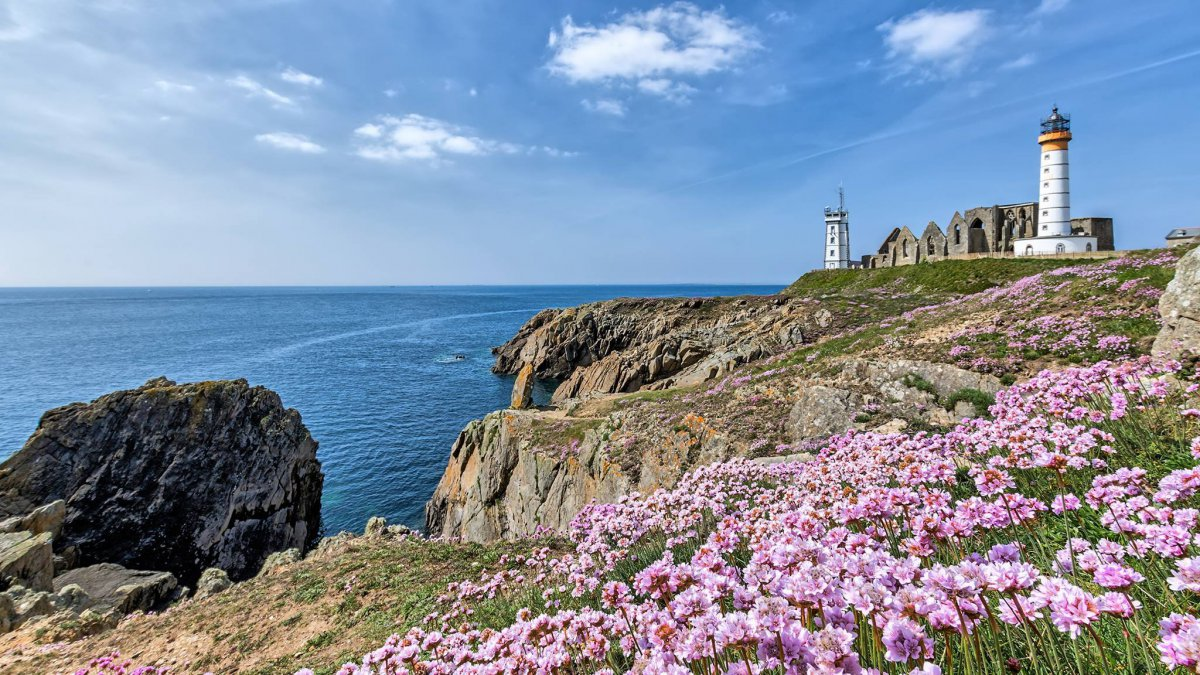
\includegraphics[width=0.7\linewidth]{Figures/saint_mathieu_avec_les_armeries_yann_quiviger-3215501}%
	\caption[Short caption goes to List of Figures]{This is a long caption; we can describe a lot of things here. For example, this photo is impressive. The shot was in Saint-Mathieu by Yann Quivig.}%
	\label{fig:test}
\end{figure}


% ------------------------------------------------------------------------------------------------------
\section{Another Section}\label{sec:another}
This is is a reference to the Chapter~\ref{chap:intro}.


\begin{table}[htb]
\caption{The effects of treatments X and Y on the four groups studied.}%
\label{tab:treatments}
\centering
\begin{tabular}{l l l}
\toprule
Groups & Treatment X & Treatment Y \\
\midrule
1 & 0.2 & 0.8\\
2 & 0.17 & 0.7\\
3 & 0.24 & 0.75\\
4 & 0.68 & 0.3\\
\bottomrule\\
\end{tabular}
\end{table}


\Blindtext%

\simplebox{%
\begin{otherlanguage}{french}
	\lipsum[4]%
\end{otherlanguage}
}

\lipsum[6]

\section{An extra section}
\Blindtext%
	
\Blindtext%

\begin{algorithm}
	\begin{algorithmic}[1]
		
		\STATE{\textbf{input:} $G$} \COMMENT{Graph}
		\STATE{\textbf{output:} $\mathcal{C}$} \COMMENT{Set  of all maximal cliques in G.}
		
		
		\STATE{adj $\leftarrow$ list all adjacent pairs in G}
		\STATE{Q $\leftarrow \emptyset$}   \COMMENT{Queue of candidates}
		
		\STATE{subg $\leftarrow$ list of all nodes in G}
		\STATE{cand $\leftarrow$ list of all nodes in G} \COMMENT{Candidates to be evaluated}
		
		\STATE{u $\leftarrow$ node in subg with highest cardinality}
		\STATE{ext\_u $\leftarrow$ list of nodes in cand except the set of adjacent of u}
		\STATE{stack $\leftarrow \emptyset$} \COMMENT{Execution stack}
		
		\WHILE{\TRUE{}}
		\IF{ext\_u $\ne \emptyset$}
		\STATE{q $\leftarrow$ POP(ext\_u)} \COMMENT{next node in the ext\_u list.}
		\STATE{cand $\leftarrow$ cand \arraybackslash {q}} \COMMENT{remove q node from cand.}
		\STATE{Q $\leftarrow$ PUSH(Q,q)} \COMMENT{Push q in the list Q.}
		\STATE{adj\_q $\leftarrow$ list of adjacent of q}
		\STATE{subg\_q $\leftarrow$ subgraph with all adjacents of q} 
		\IF{subg\_q $= \emptyset$}
		\STATE{$\mathcal{C}$ $\leftarrow$ Q}
		\ELSE{} 
		\STATE{cand\_q $\leftarrow$ set of nodes in cand adjacent to q}
		\IF{cand\_q $\ne \emptyset$}
		\STATE{stack $\leftarrow$ stack $\cup$ \{(subg, cand, ext\_u)\}}
		\STATE{Q $\leftarrow$ Q $\cup$ \{ \}}
		\STATE{subg $\leftarrow$ subg\_q}
		\STATE{cand $\leftarrow$ cand\_q}
		\STATE{u $\leftarrow$ node in subg with highest cardinality}
		\STATE{ext\_u $\leftarrow$ list of nodes in cand except the set of adjacent of u}
		\ENDIF{}
		\ENDIF{}
		
		\ELSE{}
		\STATE{POP(Q)}
		\STATE{subg, cand, ext\_u $\leftarrow$ POP(stack)}
		\ENDIF{}
		\ENDWHILE{}
		\RETURN{$\mathcal{C}$}
	\end{algorithmic}
	\caption{Output all maximal complete subgraphs.}\label{alg:fclique}	
\end{algorithm}

%\begin{algorithm}
%	\caption{test 2}
%\end{algorithm}
\subsection{Section 2}
\Blindtext%
\subsubsection{Section 2}
\Blindtext%
%\begin{algorithm}
%	\caption{test}
%\end{algorithm}

\chapter{The Second Chapter}
\Blindtext%
\section{A section here} 
\Blindtext%
\section{A subection here} 
\Blindtext%
\subsection{A subsubection here} 
\Blindtext%
\subsection{Another subsubection here} 
\Blindtext%
\subsubsection{A subsubection here} 
\Blindtext%
\addsubsubsec{A subsubection not numbered here} 
\Blindtext%



%\include{./chapters/chapter3} 
%\include{./chapters/chapter4} 
%\include{./chapters/chapter5} 
 
%----------------------------------------------------------------------------------------
%	THESIS CONTENT - APPENDICES
%----------------------------------------------------------------------------------------
%\backmatter
\tableofcontents   % Prints the main table of contents
\listoffigures     % Prints the list of figures
\listoftables  	   % Prints the list of tables
\listofalgorithms  % Prints the list of tables

%----------------------------------------------------------------------------------------
%	SYMBOLS
%----------------------------------------------------------------------------------------

\begin{symbols}{@{}p{50pt}@{}p{250pt}@{}p{50pt}} % Include a list of Symbols (a three column table)

$a$ & distance & \si{\meter} \\
$P$ & power & \si{\watt} (\si{\joule\per\second}) \\
%Symbol & Name & Unit \\

\addlinespace % Gap to separate the Roman symbols from the Greek

$\omega$ & angular frequency & \si{\radian} \\

\end{symbols}
	   % list of symbols

%----------------------------------------------------------------------------------------
%	PHYSICAL CONSTANTS/OTHER DEFINITIONS
%----------------------------------------------------------------------------------------
%lr@{${}={}$}l
\begin{constants}{@{}p{150pt}@{}p{20pt}@{}p{150pt}} % The list of physical constants is a three column table

% The \SI{}{} command is provided by the siunitx package, see its documentation for instructions on how to use it

Speed of Light & $c_{0}$ & \SI{2.99792458e8}{\meter\per\second} (exact)\\
%Constant Name & $Symbol$ & $Constant Value$ with units\\

\end{constants}
     % list of constants

% USING acro package content are in ./acro-def.tex
\ifbool{acrosupport}{%
    \printacronyms
}{% ELSE
	
%----------------------------------------------------------------------------------------
%	ABBREVIATIONS
%----------------------------------------------------------------------------------------

\begin{abbreviations}{@{}p{50pt}@{}p{250pt}} % Include a list of abbreviations (a table of two columns)

\textbf{LAH} & \textbf{L}ist \textbf{A}bbreviations \textbf{H}ere\\
\textbf{WSF} & \textbf{W}hat (it) \textbf{S}tands \textbf{F}or\\
\textbf{PDF} & \textbf{P}ortable \textbf{D}ocument \textbf{F}format\\
\end{abbreviations}
 % list of abbreviations
}

% Uncomment the lines as you write the Appendices
\addpart{Appendices}
\appendix 			% Cue to tell LaTeX that the following "chapters" are Appendices
% Appendix A
\chapter{Frequently Asked Questions}% Main appendix title
\label{AppendixA}% For referencing this appendix elsewhere, use \ref{AppendixA}

\section{How do I change the colors of links?}
The color of links can be changed to your liking using:



{\small\verb!\hypersetup{urlcolor=red}!}, or

{\small\verb!\hypersetup{citecolor=green}!}, or

{\small\verb!\hypersetup{allcolor=blue}!}.

\noindent If you want to completely hide the links, you can use:

{\small\verb!\hypersetup{allcolors=.}!}, or even better: 

{\small\verb!\hypersetup{hidelinks}!}.

\noindent If you want to have obvious links in the PDF but not the printed text, use:

{\small\verb!\hypersetup{colorlinks=false}!}.

%\include{./appendices/appendixB}
%\include{./appendices/appendixC}

%----------------------------------------------------------------------------------------
%	BIBLIOGRAPHY
%----------------------------------------------------------------------------------------
\addpart{\bibname}		% start Bibiography part
\nocite{*} 				% force to cite all entries

%\printbibliography[heading=bibintoc]
% nocite: In order to cite all the references included biblio

\printbibliography[heading=primary,keyword=primary]
\newpage
\printbibliography[heading=secondary,keyword=secondary]

\end{document}
